\documentclass[notitlepage]{article}
\usepackage[utf8]{inputenc} 
\usepackage{geometry} 		
\usepackage{chngcntr}
\usepackage{amsmath} 			
\usepackage{amssymb}			
\usepackage{mathtools}		
\usepackage{comment} 			
\usepackage{mdframed}			
\usepackage{xcolor}				
\usepackage{fancyhdr}			
\usepackage{listings}			
\usepackage{color}				
\usepackage{tikz}	
\usepackage{tasks}			
\usepackage{exsheets}		
\usepackage{array}			
\usepackage{empheq}
\usepackage{caption}
\usepackage{pdfpages}
\usepackage{tabularx}

\geometry{ 						%Format titlepage (interrupted by newgeometry)
	a4paper,
	total={170mm,257mm}%,
	%left=0mm,
	%top=0mm,
}

%START DEFINE YOUR VARIABLES HERE

\newcommand{\documentName}{Project Initiation}
\newcommand{\projectName}{Label Refinement by Behavioral Similarity}

%END DEFINE YOUR VARIABLES HERE

\title{%
	\documentName\text{ } \\
  \large \projectName\text{ } \\
  }

\author{
	\large \underline{Document owners:}\\ 
	Bianka Bakullari\\
	\texttt{}
	Christopher Beine\\
	\texttt{}
	Nicole Ventsch\\
	\texttt{}
	Juan\\
	\texttt{}
}

\date{\small{Last edited: \today}}

\pagestyle{fancy}
\fancyhf{}
\rhead{}
\lhead{\documentName\space-\space\projectName}

\makeatletter					%Prefix to add ToC to titlepage
\newcommand*{\toccontents}{\@starttoc{toc}}
\renewcommand*\contentsname{}
\makeatother
                  

\begin{document}

\begin{titlepage}
\clearpage\maketitle			%Clear title page
\thispagestyle{fancy}
\tableofcontents
\end{titlepage}

\rfoot{\thepage}				%Start printing page-numbers, after title page.

\newgeometry{ 					%Default page formatting on-going #1
	total={170mm,257mm},
	left=20mm,
	top=25mm,
    bottom=30mm					%Causes warning
}

\begin{flushleft}				%Default page formatting on-going #2

\section{Overview}
Many processes involve carrying out an action multiple times. An example for this would be an online shop in which you first have to pay a registration fee before ordering an item and paying it. This process contains the event "payment" twice, but in different contexts, so that the payments are actually two different tasks. In the context of analysing processes, the event logs usually only contain the event names, so that the "payment" actions would be treated as the same task and loops would be induced in the resulting models. However, these loops do not match the actual process, which is the issue this project addresses. 

These imprecise logs should be refined based on the structural contexts of the events. We want to refine the logs without any filtering. Moreover, we want to allow an interactive change of the thresholds used to refine the labels since this can differ for every log and we have no knowledge of the correctness of the refined log in general. All of this should be done by creating a Python-based web service in this project.




\section{Business Case}

Based on the situation explained in the overview, we now want to discuss the business case and explore the project`s potential. We will do this by first defining the scope of the project, then the assumptions we take and finally we will consider the advantages that are gained by carrying out this project. 
% \subsection{Intial situation}

\subsection{Scope}

During the project, we will create both code and documentations. Thus, the scope will be divided into these two aspects:

Documentation: 
\begin{itemize}
	\item create a Project Initiation Document 
	\item realize the Requirements Specification document
	\item develop and describe the design of the interface 
	\item design the algorithm structure by stating the usage of classes as well as the inputs and outputs for the functions that are used
	\item Software Documentation during milestones
\end{itemize} 


Implementation:
\begin{itemize}
	\item set up a Web Service based on Python that uses the label refinement algorithm proposed by Xixi Lu, et al.
	\item create a user interface that allows the users to upload the original event log, set thresholds and imprecise label scope and finally download the refined event log
\end{itemize}

For the realization of our project some background in Process Mining is needed, as well as programming knowledge.
Moreover, the documentation of both organizational aspects as well as software will follow the software development lifecycle where each part has to be submitted before the corresponding due date stated in the section "Project Plan - Milestones".


\subsection{Assumptions}

In this project we will assume that an event log is given by the user, i.e., data that contains at least the attributes "id", "time stamp" and "activity name". Moreover, we will assume that these event logs are given in the standard XES format.
Since the set of candidates for imprecise labels is given by the user, we assume that the quality of the processes applied on the refined event log also depends on the domain knowledge of the user who picks the candidate labels.
Our algorithm is a pre-processing step in itself and it does not include other preprocessing mechanisms like filtering.
In this context, instead of considering imprecise labels as noise and filtering the out, we change the labels based on the patterns present in the data.



\subsection{Key Benefits}
 
With this project we mainly aim at improving given event logs by making them more precise, so that the subsequent analysis will be more accurate. 
Our Label Refinement algorithm gives data scientists the opportunity to apply the process discovery algorithms to both original and refined event logs, leading to more alternative solutions from which the best can be chosen.
More correct models enable gaining better insights from the data, which on the other hand gives the data scientists the opportunity to take the best measures in order to optimize the processes and that way reduce the company's expenses while increasing its efficiency.  

By designing an interface that allows the users to upload an event log, to set the thresholds and to download the modified event log, carrying out this project will save the data analysts a lot of time which would be needed to refine the log themselves and also help them find better models systematically. 
By providing a web service, the software can be used on demand and there are only minor requirements for the user's hardware which avoids the necessity to stick to a given programming language or software.




\section{Feasibility study}
In this section we give a description of our project by explaining why the task is realizable from both theoretical and technical point of view.
We also try to take potential risks into account and propose countermeasures.

\subsection{Theoretical point of view}

From a theoretical point of view, we view an event log for which we suspect to have different tasks being handled as the same activity as \textit{imprecise}.
In reality, each event in the data is a unique occurrence over time.
By defining a \textit{labeling  function} which maps these events to a finite set of activity names, also called \textit{labels}, we obtain event logs having common activities across traces and within traces.
A problem arises when similar events happening in different contexts are assigned the same label.
Applying process discovery algorithms to such event logs may lead to process models being imprecise, misleading or even incorrect.

There has already been some research investigating this problem. 
Some of the approaches include using additional domain knowledge to correct the labeling, or trace clustering to do relabeling according to the different variants.

In our project, we focus on the algorithm developed, investigated and explained in \cite{paper}, which given an event log, refines the labels of events based only on the context and patterns present in this event log.
The approach consists of three main steps: 1)detecting activities which need refined labels, do relabeling 2)accross dissimilar traces and then 3)within traces.
Here we assume that the set of candidate activities needing relabeling is given and the user should have the possibility to set the thresholds affecting the relabeling in steps 2) and 3).

Since the logs have a finite set of activities leaving room for only a reduced number of computations needed for the cost function in step 2) and the fact that this algorithm has already been successfully implemented in ProM yielding good results, we conclude that the project is feasible from a theoretical point of view.\\

\subsection{Technical point of view}

As stated in \cite{paper}, the algorithm has already been implemented in ProM, where controlled experiments have been made to test the performance of the algorithm based on event logs containing different patterns.
There has also been a real life case study involving an event log with data concerning healthcare which was provided by Maastricht University Medical Center (MUMC+), a large academic hospital in the Netherlands.
In the log containing 1039 cases and 6213 events, the activities \textit{surgery} and \textit{consultation} were imprecise.
After relabeling, the resulting model reflected the behaviour which was described by the domain experts, according to whom the acitivity \textit{surgery} for example took place many times during the treatment of certain patients.
\medskip
For our project we will use following open source tools: 
\medskip
\begin{itemize}
	\item Python 3.7.2 as back-end programming language
	\item pm4py python library as process mining toolkit
  \item NetworkX pyhton library for graph manipulation
  \item Flask 1.0.2 as web application framework
	\item JavaScript as Front-end development language (Standard ECMAScript 2018)
\end{itemize}

We will seperate the application into two main parts the back-end which is responsible for the algorithm and API design and the front-end to provide a user friend interface.\\
\medskip
Python is used as back-end programming language to implement the algorithm. Additionally, we will use Flask as a lightweight webapplication framework. 
It provides a quick start and is easily customizable via plug-ins. It is also used in enterprise applications like Netflix Lemu [?].\\
\medskip
In particular we will make use of the .pm4py library which is a joint effort of the Process Mining group at the Fraunhofer FIT and the Chair of
RWTH Process and Data Science group as it supports many process mining algorithms and performance measures in Python.\\
\medskip
The frontend is for visualization only. It is created with HTML5 and JavaScript to access the API and to perform ui logic. 
Thus, presentation and business logic can be easily separated and replaced.\\
\medskip
The final web application will be optimized for Google Chrome (Version $\geq$ 65) and Firefox (Version $\geq$ 60).


\subsection{Risks and mitigations}
In the following we try to estimate the potential problems and risks that may arise during our project and propose ways to be prepared for or overcome them.
We take into consideration complications concerning the organisational and management aspects, as well as those arising when implementing the algorithm.

\subsubsection{Project management risks}

\begin{tabularx}{15cm}{|X|X|}
\hline
\textbf{Risks} &\textbf{Mitigations}\\
\hline
Misunderstanding of tasks & Do regular discussions, meetings in the group and with the project supervisor\\
\hline
Unmatching schedules of the team members & Arrange meetings in advance, notify other members for any change  \\
\hline
Acquiring new skills under time pressure & Assign tasks based on individual strengths to increase efficiency \\ 
\hline
\end{tabularx}\\ 


\subsubsection{Technical risks}

\begin{tabularx}{15cm}{|X|X|}
\hline
\textbf{Risks} &\textbf{Mitigations}\\
\hline
Inconsistencies in programming styles & Explain the code to other members, write useful comments while coding\\
\hline
Unclear performance measures & Test code on small event logs, use automatically generated event logs to experiment \\
\hline
Software components do not work as a whole & Put emphasis on the design step \\ 
\hline
\end{tabularx}



\section{Project Plan}

\subsection{Milestones}

The project starts on the 09/04/2019 and ends on the 08/07/2019 and is divided into nine milestones. The project is managed with a scrum-oriented approach
where each milestone represents a sprint. The project team organizes the required tasks during each sprint and visualize the current project status via a dashboard.

\begin{center}
	\captionof{table}{Overview Milestones }
  \begin{tabular}{ m{0.4cm} m{5cm} m{8.5cm} m{2cm} }
  	\hline
		ID & Milestone & Description & Deadline \\ \hline
		1 & Project Initiation document & The Project Initiation Document provides all of the key information required to start and run the project. This includes the project description, business case, feasibility study and a project team presentation.  & 19/04/2019 \\ \hline
		2 & Requirements Specification document & The Requirements Specification document contains functional and none functional requirements such as a set of use cases to describe the system interactions. & 29/04/2019 \\ \hline
		3 & Design Analysis and dummy P.o.C. & The final document is a description about the planned system architectural background and a proof of concept visualizing the main UI components. & 13/05/2019 \\ \hline
		4 & Sprint 1 code and documentation & In this sprint the import module and a static frontend will be implemented.  & 24/05/2019 \\ \hline
		5 & Sprint 2 code and documentation & In this sprint the algorithm will be implemented. & 07/06/2019 \\ \hline
		6 & Sprint 3 code and documentation & IN this sprint the final user interface and visualization will be implemented. & 21/06/2019 \\ \hline
		7 & Testing, assessment and deployment & The application is checked for accuracy and should be aviable for use. & 01/07/2019 \\ \hline
		8 & Final report on the project & The final report provides an overview about the project course and the result. & 08/07/2019 \\ \hline
	\end{tabular}
\end{center}

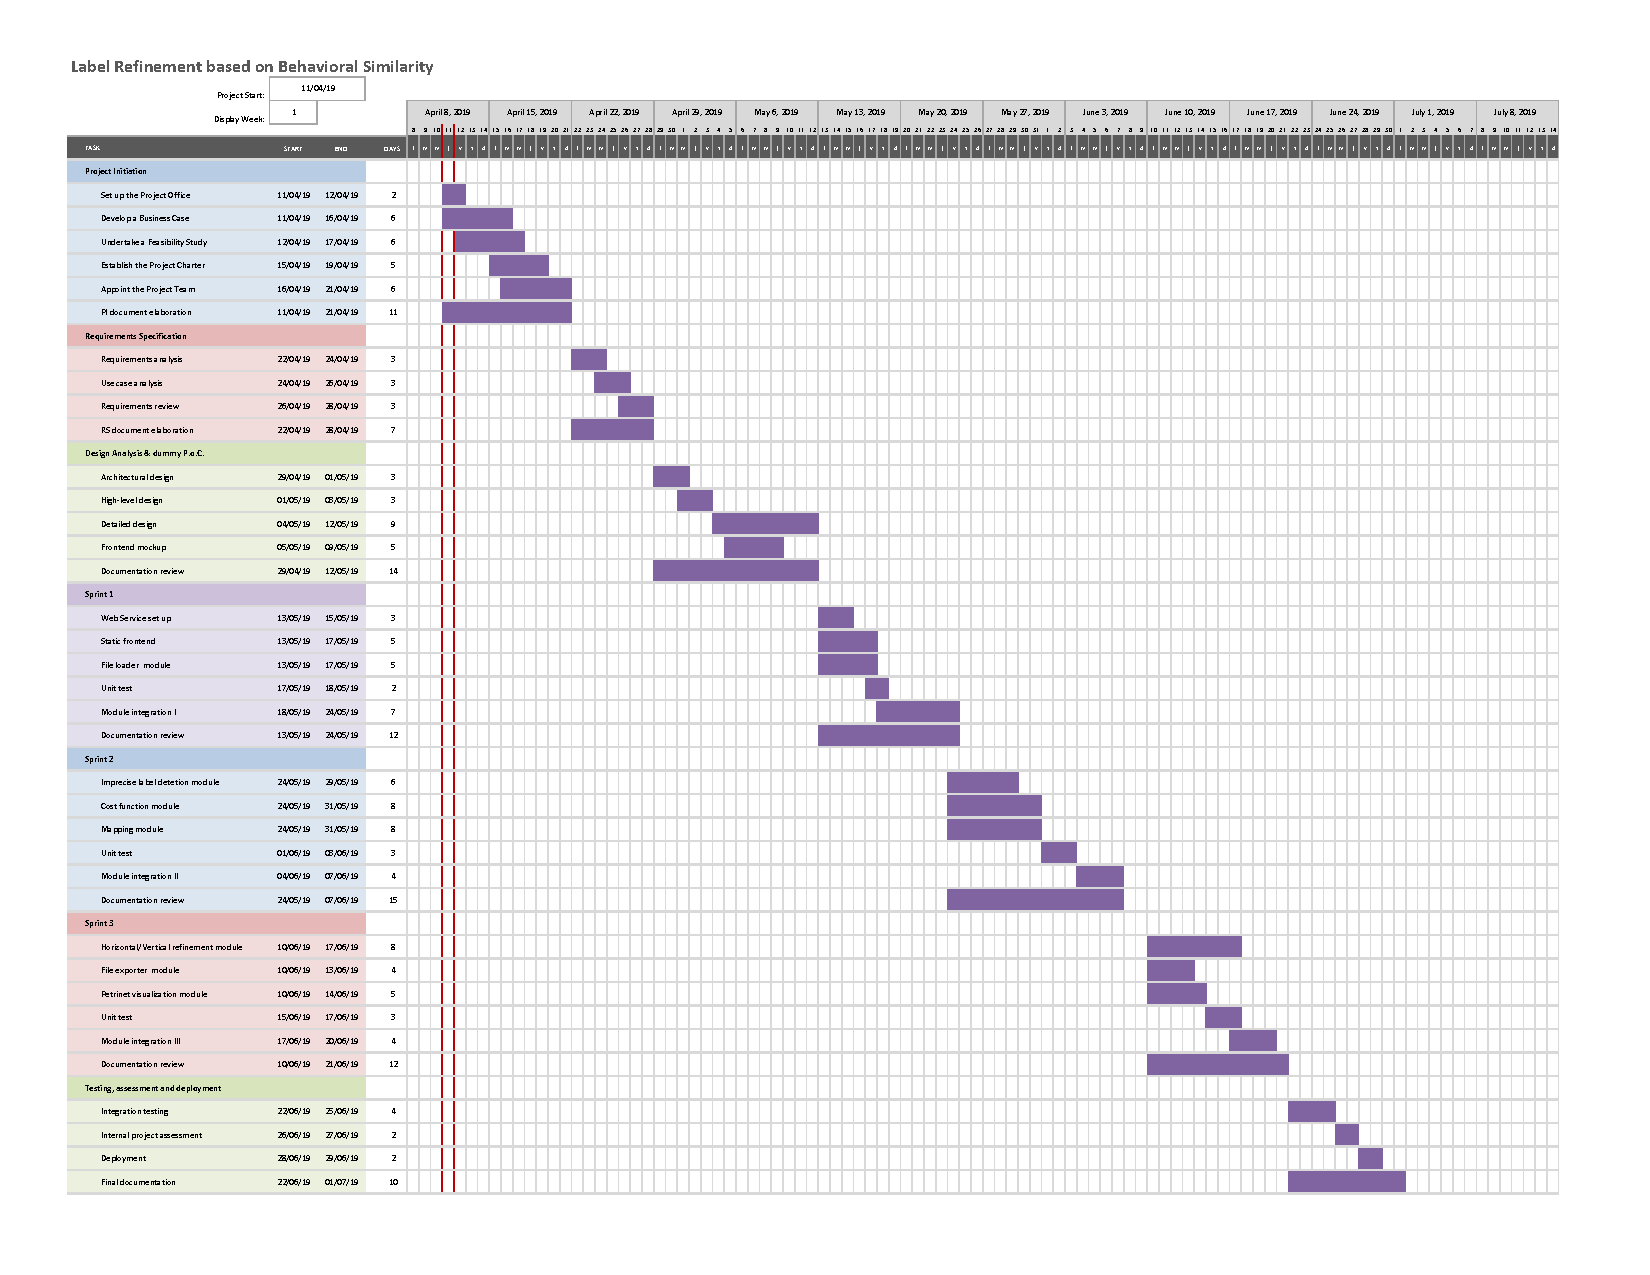
\includepdf[landscape=true]{ganttChart.pdf} 

\subsection{Deliverables}
With each milestones various deliverables are created to monitor, document and verify the docuemnt progress.
\newline
\textbf{1 Project Initiation document:}
\\
\begin{itemize}
	\item Finale project initiation document with key information about the project
\end{itemize}

\textbf{2 Requirements Specification document:}
\\
\begin{itemize}
	\item Requiredments Specification document with functional und none functional requirements
	\item Use case analysis
\end{itemize}

\textbf{3 Design analysis and dummy P.o.C:}
\\
\begin{itemize}
	\item System and software architecture documentation
	\item Frontend mockup
\end{itemize}

\textbf{4 Sprint 1 code and documentation }
\\
\begin{itemize}
	\item Unit Test protocols
	\item Code documentation
\end{itemize}

\textbf{5  Sprint 2 code and documentation }
\\
\begin{itemize}
	\item Unit Test protocols
	\item Code documentation
\end{itemize}

\textbf{6 Sprint 3 code and documentation }
\\
\begin{itemize}
	\item Unit Test protocols
	\item Code documentation
\end{itemize}

{\color{red} @all: should we write tests during the implementation? Could possibly save us a lot of trouble, but we have to select a test framework.
Otherwise we can remove the Unit Test protocols}

\textbf{7 Testing, assessment and deployment}
\\
\begin{itemize}
	\item Testprotocols
	\item Server configuration
	\item Web API 
	\item Webapplication
\end{itemize}

\textbf{8 Final report on the project}
\\
\begin{itemize}
	\item Final report
\end{itemize}

{\color{red} @all: Any other documents, reports, protocols or code artefacts required?}

\subsection{Timetable}

\section{Project Team}
In the following we focus on the individual strengths of the members of the team and specify the responsibilities with respect to the milestones of the project.

\subsection{Competences} 
In this section we introduce the members of our team by shortly describing their knowledge and competences which will be useful to carry out the task successfully.

\subsubsection*{Nicole Ventsch}

Nicole Ventsch is a Master student at RWTH studying Mathematics and Data Science in parallel. She is studying both subjects in her second semester of the master's degree. Moreover, she works as a student assistant in the field of Data Analytics / Business Intelligence. Due to her background in mathematics, she has a good understanding of theoretical foundations. Moreover, she is very interested in Data Science and already took many courses in that area. Since she took the course "Introduction to Data Science", she has also worked with Python before. Though she has a strong theoretical background, she has never worked on user interfaces or with web services, so that this aspect of the project could be challenging for her. Additionally to that, she is not used to the software development Lifecycle, so that executing this project will include many new experiences to her. 

\subsubsection*{Juan Garza}

Juan Garza is a student at the RWTH University. He is currently in his 4th semester of studies towards a master’s degree in Computer Science. During his studies, he deepened his knowledge of process mining by attending the lecture “Business Process intelligence”. Moreover, he carried out a seminar on “Selected Topics in Process Mining”. He is familiar with Java and Python as programming languages. Besides school projects, he has no programming experience in “real world” environments which may represent a difficulty for him. 

\subsubsection*{Bianka Bakullari}

Bianka Bakullari is a Master student at RWTH studying Computer Science.
She has a good theoretical background on the field of Process Mining after having attented the lectures "Business Process Intelligence" and "Introduction to Data Science". 
Currently she is attending the "Advanced Process Mining" lecture.
She has gathered some experience working with Python where in most cases pre-processing and analysis was made on concrete event data, therefore a challenge of this project is implementing an algorithm that works on any given event log efficiently.
Since she has never worked with web applications before so the execution of this step will be a new experience for her.


\subsubsection*{Christopher Beine}
Christopher Beine is a 4th semester Bachelor student at the RWTH Aachen University. Before his studies, he made an apprenticeship as a Computer Science Expert Subject Area: Software Development 
by Phoenix Contact GmbH \& Co. KG where he works as a full-stack developer. He supervised several software projects within the company and is currently 
developing a web application for planning and visualizing the strategic orientation. In the field of data science, he deepens his knowledge with online courses such as the "Machine Learning" from Standford University on Coursera. 
He has practical experience with C\#, PHP, JavaScript, the software development lifecycle and the most common web technologies.    


\subsection{Roles}
We emphasize that all of the team members are supposed to put active effort on each of the milestones of the project.
However, we assign a team member to have main responsibility for each step in order to ensure that the deliverables have sufficient quality and nothing is missing.

\begin{center}
  \begin{tabular}{ m{0.4cm} m{5cm} m{5cm} m{6cm} }
  	\hline
		ID & Milestone & Chief Responsibility & Contact \\ \hline
		1 & Project Initiation document & Bianka Bakullari & bianka.bakullari@gmail.com \\ \hline
		2 & Requirements Specification document & xx & yy \\ \hline
		3 & Design Analysis and dummy P.o.C. & Christopher Beine & christopher.beine@rwth-aachen.de \\ \hline
		4 & Sprint 1 code and documentation & xx  & yy \\ \hline
		5 & Sprint 2 code and documentation & Bianka Bakullari & bianka.bakullari@gmail.com \\ \hline
		6 & Sprint 3 code and documentation & Christopher Beine & christopher.beine@rwth-aachen.de \\ \hline
		7 & Testing, assessment and deployment & xx & yy \\ \hline
		8 & Final report on the project & xx & yy \\ \hline
	\end{tabular}
\end{center}













\section{Project office}

In order to better be able to keep track of our progress, we use the Trello dashboard to divide our tasks into planned, running and completed ones.
Trello also gives the opportunity to write descriptions and comments on each task, so that everyone is able to specify certain things needed to be considered or problems having arised.
For our deliverables we use Git, as this makes it able to keep track of any changes and updates to our documentation or code.
All members and the instructors have access to both Trello account and Git repository.

%\newpage
%\bibliographystyle{plain}
%\bibliography{references}  




\addcontentsline{toc}{chapter}{\textbf{References}}
\end{flushleft}
%\bibliography{uw-ethesis}
% Tip 5: You can create multiple .bib files to organize your references. 
% Just list them all in the \bibliogaphy command, separated by commas (no spaces).

% The following statement causes the specified references to be added to the bibliography% even if they were not 
% cited in the text. The asterisk is a wildcard that causes all entries in the bibliographic database to be included (optional).


\begin{thebibliography}{5}
\bibitem{paper}
Lu, Xixi, et al. "Handling duplicated tasks in process discovery by refining event labels." International Conference on Business Process Management. Springer, Cham, 2016.










\end{thebibliography}










\end{document}
